\subsubsection{Влияет ли на величину выходного напряжения ёмкость сглаживающего конденсатора, устанавливаемого на выходе выпрямителя? Каково это напряжение?}

Рассмотрим простейший 1 п/п выпрямитель со сглаживающим конденсатором на выходе.
\begin{center}
	\begin{figure}[h!]
		\center{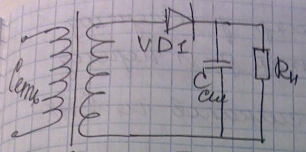
\includegraphics[scale=0.7]{1ppc.png}}
		\caption{}	
	\end{figure}
\end{center}

В первый полупериод конденсатор $C = C_{s}$ заряжается до величины входного сигнала с учётом потерь($R_g$ и т.п.). А во второй разряжается через $R_{out}$(т.к. диод закрыт).

После переходного процесса установится примерно следующая картина для выходного напряжения: 
\begin{center}
	\begin{figure}[h!]
		\center{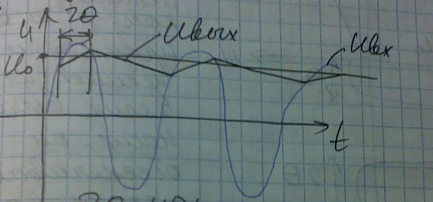
\includegraphics[scale=0.7]{1ppcU.png}}
		\caption{}	
	\end{figure}
\end{center}

В течение времени $2\Theta$ диод открыт и  происходит зарядка конденсаора. У Пилообразного выходного напряжения можно выделить среднее значение, которое будет равно 
$$
U_0 = U_m\cos\Theta
$$
$\Theta$ можно найти из уравнения:
$$
tg\Theta - \Theta = \frac{\pi r_{\textit{потерь}}}{mR_{out}}
$$
m = 1,2 для одно и двух полупериодных выпрямителей.

Когда диод открыт, конденсатор заряжается через $R_g$ и диод с постоянной времени
$$
\tau_{zar} = C(R_g + r_{dif})
$$

Когда диод закрыт, конденсатор разряжается через $R_{out}$(сопротивление обратно включенного диода примем большим).

На ВАХ развертка сигналов выглядит примерно следующим образом:
\begin{center}
	\begin{figure}[h!]
		\center{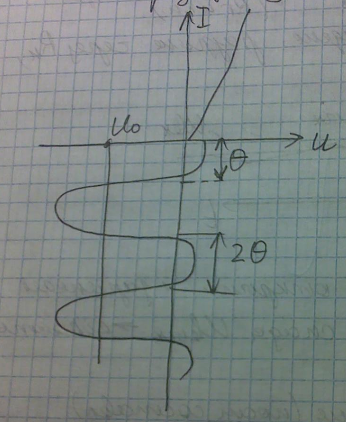
\includegraphics[scale=0.7]{razv.png}}
		\caption{}	
	\end{figure}
\end{center}

Таким образом, конденсатор обеспечивает сглаживание пульсаций. Его величина практически не влияет на величину среднего выходного напряжения.
\pagebreak
